\documentclass[times, utf8, seminar, numeric]{fer}
\usepackage{booktabs}
\usepackage{listings}
\usepackage{color}
\usepackage{url}
\usepackage{amsmath}
\usepackage{color, colortbl}
\usepackage[group-separator={,}]{siunitx}

\definecolor{mygreen}{rgb}{0,0.6,0}
\definecolor{mygray}{rgb}{0.5,0.5,0.5}
\definecolor{mymauve}{rgb}{0.58,0,0.82}
\definecolor{gray1}{rgb}{0.87,0.87,0.87}
\definecolor{gray2}{rgb}{0.96,0.96,0.96}

\lstset{ %
  backgroundcolor=\color{white},   % choose the background color
  basicstyle=\footnotesize,        % size of fonts used for the code
  breaklines=true,                 % automatic line breaking only at whitespace
  captionpos=b,                    % sets the caption-position to bottom
  commentstyle=\color{mygreen},    % comment style
  escapeinside={\%*}{*)},          % if you want to add LaTeX within your code
  keywordstyle=\color{blue},       % keyword style
  stringstyle=\color{mymauve},     % string literal style
}

\begin{document}

\title{Očitavanje rukom pisanih slova}
\author{Filip Gulan}
\voditelj{doc. dr. sc. Marko Čupić}

\maketitle

\tableofcontents

\chapter{Uvod}
Očitavanje slova je problem koji se rješava već dugi niz godina. Još od 1980-ih godina, početkom ere računala, počeli su se razvijati prvi programi koji bi zamijenili čovjeka u raznim operacijama, pa tako i u očitavanju slova. Primjena je bila razna, od očitavanja brojeva računa u bankama do očitavanja poštanskih brojeva prilikom sortiranja pisama.

Svi ti sustavi su većinom bili namijenjeni za očitavanje tiskanih brojeva. Postojala je nekolicina sustava i za očitavanje rukom pisanih brojeva no oni su zahtijevali točno određene načine pisanja kako bi mogli ispravno raditi.

Razvojem računala i tehnika strojnog učenja, navedeni su poslužili prilikom izgradnje sustava za očitavanje znakova. Tako danas imamo raznorazne komercijalne alate koji bez većih problema mogu vrlo brzo i efikasno očitati cijele stranice tiskanoga tekstualnoga dokumenta.

No, očitavanjem rukom pisanih slova danas još uvijek nije unaprijeđeno na razinu točnosti kojom ljudi prepoznaju pojedina slova. Pokazalo se da najbolje rezultate prilikom prepoznavanje rukom pisanih slova ostvaruju sustavi izgrađenih na raznoraznim modelima strojnog učenja.

Kod pristupa gdje se koriste modeli strojnog učenja dolazi do nekoliko ključnih problema. Prvi od njih je skup za učenje koji treba biti skupljen od velikog broja ljudi kako bi izgrađeni sustav bio što bolje otporan na različite rukopise. Drugi problem je veličina samog skupa za učenje, jer što je skup veći, to je klasifikatora računski zahtjevnije za naučiti. Također, kod navedenoga pristupa postoji problem što klasifikator naučen za jedno pismo, neće raditi ispravno za drugo pismo, na primjer sustav za očitavanje latiničnih znakova neće raditi ispravno prilikom očitavanja kineskih slova.

Kroz ovaj rad prikazat će se izgradnja takvog sustava kroz prizmu dubokog učenja i konvolucijskih neuronskih mreža.



\chapter{Konvolucijske neuronske mreže}
Obične neuronske mreže najčešće su sastavljene od jednog ulaznog, jednog izlaznog te jednog ili više skrivenih slojeva. Neuronska mreža na ulaznom sloju prima \emph{n}-dimenzijski vektor, transformira ga kroz niz skrivenih slojeva te na izlaznom sloju daje \emph{k}-dimenzijski vektor. Svaki sloj se sastoji od niza neurona, gdje težinske ulaze u pojedini neuron najčešće čine izlazi svih neurona iz prethodnog sloja - takvi slojevi neurona se u literaturi nazivaju potpuno povezani slojevi. 

Konvolucijske neuronske mreže \engl{ConvNet, CNN} su vrlo slične običnim neuronskim mrežama te se mogu promatrati kao nadogradnja nad njima. Konvolucijske neuronske mreže, kao i obične neuronske mreže, se sastoje od jednog ulaznog, jednog izlaznog te jednog ili više skrivenih slojeva. No, ono što razlikuje konvolucijske neuronske mreže od običnih su specifični slojevi koji čine takvu mrežu: konvolucijski slojevi i slojevi sažimanja. Najčešće arhitekture konvolucijske neuronske mreže na svom ulazu imaju jedan ili više konvolucijskih slojeva iza kojih slijedi sloj sažimanja te zatim opet niz kombinacija konvolucijskog sloja te sloja sažimanja. Mreža najčešće završava s jednim ili više potpuno povezanih slojeva.

Arhitektura neuronskih mreža koju čine konvolucijski slojevi prilagođena je za rad sa slikama i kao takva se pokazala iznimno uspješnom prilikom izrade sustava za klasificiranje slika te izlučivanje značajki iz istih \citep{Lecun1998}. Sama ideja konvolucijskih neuronskih mreža poznata je još od 60-ih godina prošlog stoljeća, dok je prva uspješna uporaba konvolucijskih neuronskih mreža bila 1990-ih godina u sustavima za čitanje poštanskih brojeva i znamenaka za čiju je implementaciju zaslužan Yann LeCunn \citep{StanfordCS}. Na slici \ref{fig:lenet5} je prikazana arhitektura konvolucijske neuronske mreže koja se koristila u navedenom sustavu te je nosila ime \emph{LeNet-5}.

\begin{figure}[htb]
    \centering
    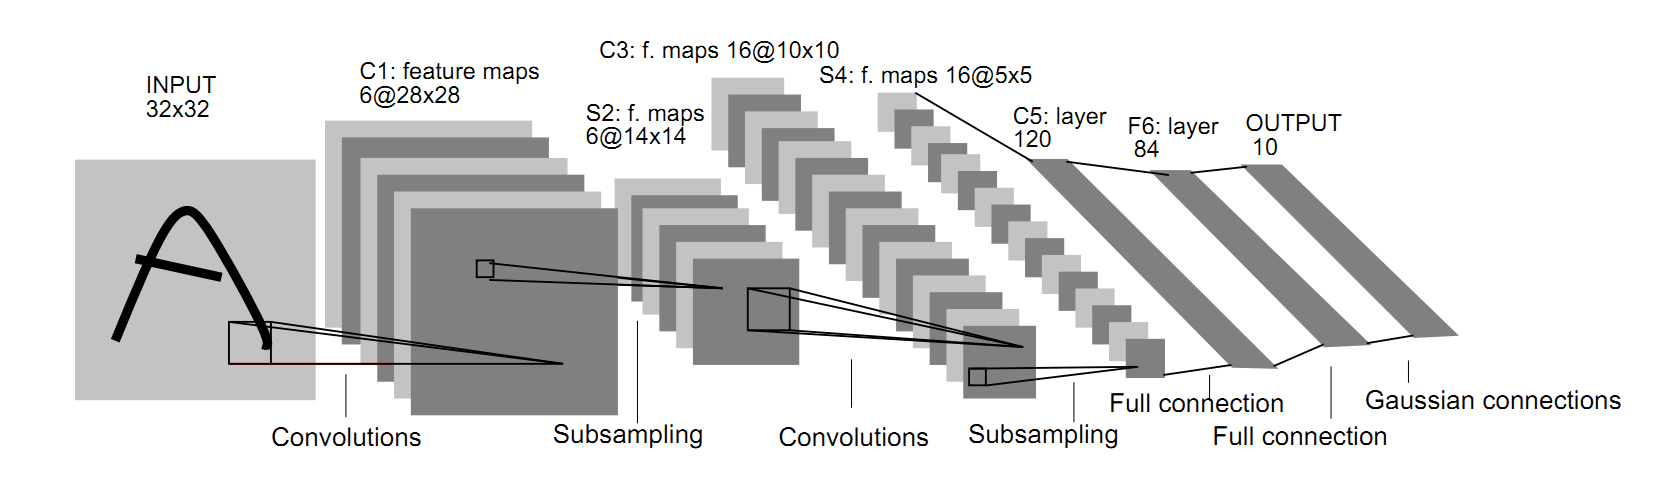
\includegraphics[width=14.5cm]{images/lenet-5.png}
    \caption{Konvolucijska neuronska mreža \emph{LeNet-5}, preuzeto iz \citep{Lecun1998}}
    \label{fig:lenet5}
\end{figure}

Kroz sljedećih nekoliko potpoglavlje bit će objašnjena uloga konvolucijskog sloja, sloja sažimanja te potpuno povezanoga sloja.

\section{Konvolucijski sloj}

Konvolucijski sloj, kako mu i ime govori, predstavlja jezgru same funkcionalnosti konvolucijske neuronske mreže. Svaki konvolucijski sloj se sastoji od filtra čije je težine potrebno podesiti to jest naučiti u fazi učenja neuronske mreže. Svaki filtar je predstavljen kao prostorna matrica dimenzija $w \times h \times d$ gdje $w$ označava širinu, $h$ visinu te $d$ dubinu filtra. Širina i visina filtra su najčešće manjih prostornih dimenzija od ulaza, dok je dubina filtra uvijek jednaka dubini ulaza. Na primjer, ukoliko se mreža koristi za klasificiranje slika u boji, točnije slika s tri komponente boja, tada bi dubina filtra bila tri, to jest filtar bi činile tri matrice dimenzije $w \times h$, odnosno jedna za svaku komponentu boje.

Izlaz konvolucijskog sloja predstavlja niz aktivacijskih mapa, to jest dvodimenzionalnih matrica. Pojedina aktivacijska mapa predstavlja odziv jednog filtra koja se dobiva tako što se filtar konvoluira s ulaznim prostorom. Konvoluiranje filtra s ulazom se može predstaviti kao pomicanje filtra za određeni korak po ulaznom prostoru te računanje skalarnog umnoška između težina filtra i vrijednosti ulaza za svaku poziciju. Prilikom učenja mreže težine filtra će se podesiti tako da se pojedini filtar ''aktivira'' na mjestima gdje uoči određene značajke poput rubova, nakupine boja pa čak i kružnih oblika u višim slojevima. Primjer konvolucije ulaza filtrom dan je na slici \ref{fig:conv_example} gdje prva matrica predstavlja ulazni prostor, druga filtar te zadnja aktivacijsku mapu.

\begin{figure}[htb]
    \centering
    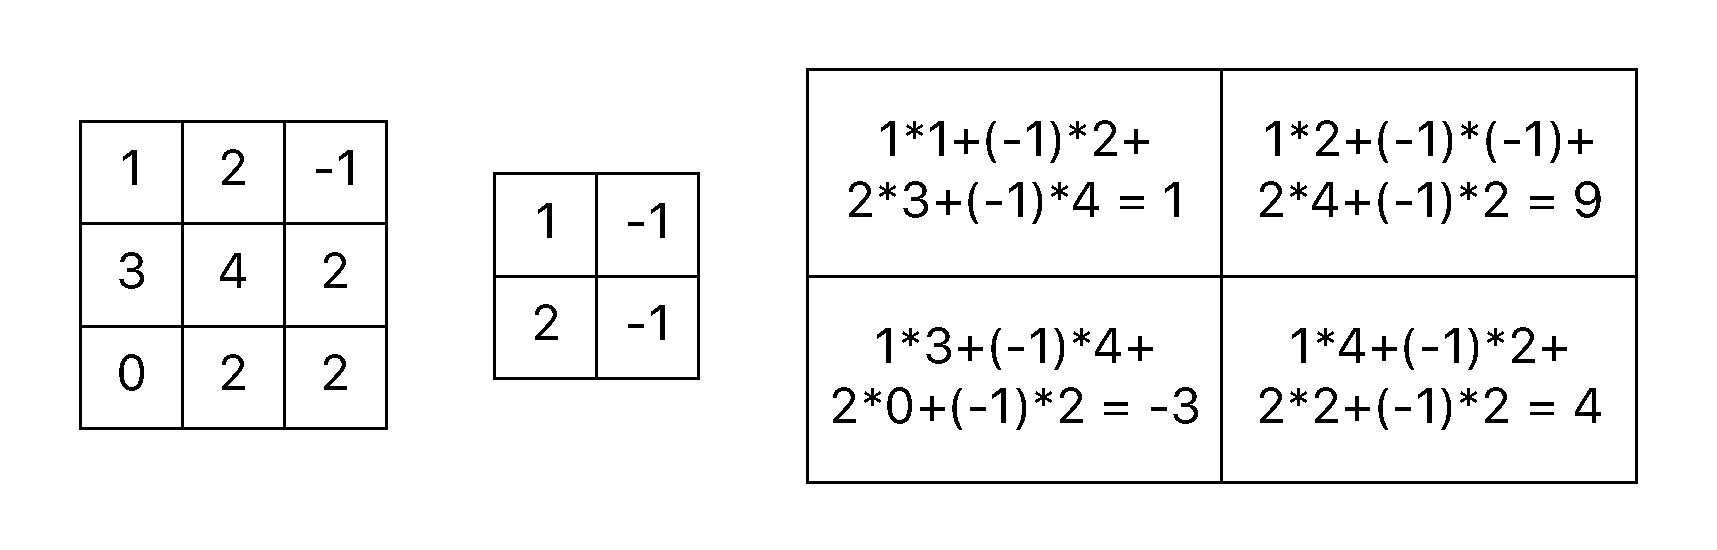
\includegraphics[width=14.5cm]{images/conv_example.pdf}
    \caption{Primjer konvolucije ulaza filtrom}
    \label{fig:conv_example}
\end{figure}

Veličina izlaza pojedinog konvolucijskog sloja definirana je s tri hiperparametara: brojem filtra, veličinom filtra te korakom pomaka filtra \engl{stride}. Korak pomaka filtra određuje za koliko koraka će se filtar pomicati po širini i visini ulaznog prostora u fazi konvolucije. Uz pretpostavku kvadratnoga filtra, da su mi širina i visina jednaki, što i je najčešći slučaj u praksi, veličina izlaza $W_o$ se može definirati izrazom \eqref{eq:conv_out}, gdje $W_i$ označava veličinu ulaza, $F$ veličinu filtra te $S$ korak pomaka filtra.
\begin{equation} \label{eq:conv_out}
W_o = \frac{W_i - F}{S} + 1
\end{equation}

Za razliku od potpuno povezanoga sloja, gdje je svaki izlaz spojen sa svim ulazima sljedećeg sloja, kod konvolucijskog sloja svaki izlaz je spojen samo sa malim dijelom ulaza sljedećeg sloja što dovodi do puno manje veza, a samim time i puno manje težina, to jest parametara koje je potrebno naučiti.

Često se u praksi izlazi konvolucijskog sloja, to jest vrijednosti aktivacijskih mapa, ''provlače'' kroz aktivacijsku funkciju danu izrazom \eqref{eq:relu}, koja se u literaturi naziva \emph{ReLU} \engl{rectified linear unit}.
\begin{equation} \label{eq:relu}
f(x) = max(0, x)
\end{equation}

\section{Sloj sažimanja}

Nakon jednog ili više konvolucijskih slojeva često dolazi i sloj sažimanja. Cilj navedenoga sloja je smanjenje prostornih dimenzija ulaza, odnosno aktivacijskih mapa. Smanjenjem prostornih dimenzija ulaza ovaj sloj zapravo kontrolira i smanjuje mogućnost prenaučenosti mreže jer povećava invarijantnost na pomak, to jest neosjetljivost na manje pomake značajki u ulaznom prostoru što je vrlo korisno u slučaju kada je za raspoznavanje bitnije utvrditi prisutnost određene značajke, nego njezinu točnu lokaciju.

U literaturi postoji nekoliko vrsti sažimanja: sažimanje srednjom vrijednosti, sažimanje maksimalnom vrijednosti, sažimanje L2 normom te sažimanje težinskim usrednjavanjem. U praksi se najčešće koristi sažimanje maksimalnom vrijednosti i to s filtrima dimenzija $2 \times 2$ koji ukupno odbacuju $75\%$ vrijednosti ulaza. Primjer takvog sažimanja dan je na slici \ref{fig:pool_example}.

\begin{figure}[htb]
    \centering
    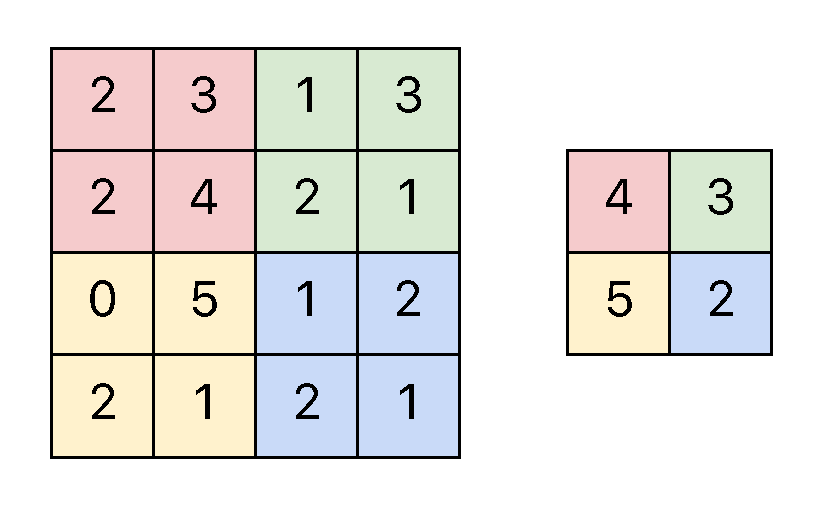
\includegraphics[width=7.5cm]{images/pool_example.pdf}
    \caption{Primjer sažimanja maksimalnom vrijednosti}
    \label{fig:pool_example}
\end{figure}

Bitno je uočiti kako sloj sažimanja utječe na smanjenje širine i visine ulaznog prostora, no ne i njegove dubine, to jest broja komponenti.

\section{Potpuno povezani sloj}

Kod potpuno povezanoga sloja ulaz pojedinog neurona je spojen s izlazima svih neurona iz prethodnog sloja te se sloj kao takav ne razlikuje onome iz obične neuronske mreže. Kod konvolucijskih neuronskih mreža jedan ili više potpuno povezanih slojeva dolaze na samom kraju mreže te njihova uloga je sama klasifikacija. Stoga, konvolucijske mreže se mogu rastaviti na dva dijela: prvi dio čine konvolucijski slojevi te slojevi sažimanja, a drugi dio potpuno povezani slojevi. Prvi dio mreže se može promatrati kao sustav za izlučivanje značajki, dok se drugi dio može promatrati kao obična neuronska mreža, to jest klasifikator.

\chapter{Slični radovi}
Na temu očitavanja rukom pisanih slova izgrađena je nekolicina različitih sustava. Sustavi objavljeni u starijim radovima najčešće koriste stroj s potpornim vektorima \engl{Support Vector Machine} kao klasifikator uz prilagođene jezgre, dok noviji radovi na istu temu većinom koriste tehnike dubokog učenja te konvolucijske neuronske mreže.

\section{\emph{LeNet-5} za očitavanje slova engleske abecede}

U radu \citep{lenet5hecr} opisan je sustav za očitavanje rukom pisanih slova engleske abecede korištenjem modificirane verzije \emph{LeNet-5} konvolucijske neuronske mreže prikazane na slici \ref{fig:lenet5}. Sama mreža se razlikovala od standardne \emph{LeNet-5} arhitekture u tome što je imala veći broj neurona u pojedinim slojevima te izmijenjene veze između pojedini slojeva, točnije između dva početna konvolucijska sloja gdje je pojedini ulaz drugog konvolucijskog sloja spojen na više aktivacijskih mapa, to jest izlaza, prvog konvolucijskoga sloja.
 
Nakon određenog broja epoha, greška klasifikacije prilikom učenja mreže opada sve sporije ili čak uopće ne opada. Razlog tomu je što nakon velikog broja epoha učenja mreže, u skupu za treniranje je jako mali broj krivo klasificiranih primjera čiji je utjecaj na učenje same mreže neprimjetan. Kako bi se doskočilo tom problemu, u ovom radu je razvijen algoritam \emph{ESRL} \engl{Error-Samples-Reinforcement-Learning algorithm}.

Ideja iza tog algoritma je dinamička rekonstrukcija skupa za učenje nakon što greška klasifikacije na skupu za provjeru počne sporije opadati. Skup za učenje je rekonstruiran svakih nekoliko epoha na način da se krivo klasificirani primjeri umnože primjenom afinih transformacija i dodavanjem šuma, ili izbacivanjem dobro klasificiranih primjera tako da broj krivo klasificiranih primjera čini $33\% - 40\%$ udjela skupa za učenje.
 
 Navedeni sustav je učen i evaluiran na \emph{UNIPEN} skupu podataka velikih i malih rukom pisanih slova engleske abecede. Sustav je ostvario $93.7\%$ točnosti na skupu za testiranje za velika slova, te $90.2\%$ točnosti na skupu za testiranje za mala slova.
 
 %\section{Opuštena konvolucijska neuronska mreža}

 
 %U radu \citep{rcnn}.

\chapter{Učenje i rezultati}
Za potrebe ovog rada izgrađen je sustav za klasifikaciju rukom pisanih slova hrvatske abecede koji se temelji na konvolucijskoj neuronskoj mreži. Sama mreža je izgrađena, učena i evaluirana korištenjem biblioteke \emph{Keras}. \emph{Keras} je biblioteka pisana u programskom jeziku \emph{Python} koja nudi vrlo jednostavno programsko sučelje za izgradnju neuronskih mreža i širok spektar algoritama za učenje iste.

\section{Skup podataka}

Za potrebe učenja klasifikatora, to jest konvolucijske neuronske mreže, prikupljen je skup podataka od \num{16000} slika slova hrvatske abecede i znakova, i to \num{7750} velikih i \num{7750} malih slova te \num{500} primjera znaka "-" koji bi služio kao oznaka poništavanja odgovora ukoliko bi se navedeni sustav koristio prilikom ispravljanja ispita s abc-pitalicama.

Skup podataka je podijeljen na 63 razreda, gdje svaki razred određuje jedan znak. Pa su tako iz hrvatske abecede izbačena slova koja se mogu dobiti kombinacijom više znakova (lj, nj i dž) te su, uz spomenuti znak "-", dodana i slova engleske abecede (x, y, w i q).

Prikupljanje skupa podataka se obavljalo preko predefiniranih obrazaca gdje je svaka osoba trebala upisati po deset varijanti malog slova, te deset varijanti velikog slova što ukupno daje 640 znakova po osobi. Obrasci su skenirani u nijansama sivih boja te su se zatim sva slova automatizirano izrezivala i svrstavala u određeni razred.

Na tako izlučenom skupu slika slova obavljalo se pretprocesiranje i to u sljedećim koracima:

 \begin{enumerate}
   \item binarizacija slike slova koristeći \emph{Otsu-ovu} metodu, 
   \item segmentacija slova od ruba do ruba tako da se izbaci što veći dio pozadine te
   \item skaliranje tako izvučenog slova na dimenzije $30 \times 30$ slikovnih elemenata uz očuvanje omjera širine i visine slova.
 \end{enumerate}

Primjer obrađenih slova iz skupa podataka se može vidjeti na slici \ref{fig:dataset_example}.

\begin{figure}[htb]
    \centering
    
\includegraphics[width=11.5cm]{images/dataset_example.pdf}
    \caption{Primjer obrađenih slova iz skupa podataka.}
    \label{fig:dataset_example}
\end{figure}

\section{Arhitektura mreže}

Kako je navedeno u prijašnjem potpoglavlju, krajnja veličina slike slova je $30 \times 30$ slikovnih elemenata, stoga i mreža korištena u ovom radu na svom prvom sloju ima $900$ ulaznih točaka. Na svom izlazu mreža ima $32$ neurona. Broj izlaza je manji nego broj samih razreda slova (velikih i malih) zbog toga što navedeni sustav na izlazu ne razlikuje velika i mala slova, na primjer veliko slovo A i malo slovo a klasificira u isti razred. Razlog takvog ''pojednostavljenja'' klasifikacije leži u tome što mreža na svom ulazu dobiva čistu sliku slova, bez poznavanja konteksta u kojem se to slovo pojavilo pa bi samoj mreži bilo iznimno teško, pa čak i nemoguće, razlučiti radi li se na primjer o velikom slovu O ili malom slovu o.

Prilikom učenja klasifikatora isprobano je nekoliko različitih arhitektura konvolucijskih neuronskih mreža, no najbolji rezultati su ostvareni uz arhitekturu kod koje je poredak pojedinih slojeva bio sljedeći:

\begin{enumerate}
    \item ulazni konvolucijski sloj s $32$ filtra dimenzije $3 \times 3$ i korakom pomaka jednakim $1$, uz korištenje \emph{ReLU} aktivacijske funkcije,
    \item sloj sažimanja maksimalnom vrijednosti uz veličinu filtra $2 \times 2$,
    \item konvolucijski sloj s $64$ filtra dimenzije $3 \times 3$ i korakom pomaka jednakim $1$, uz korištenje \emph{ReLU} aktivacijske funkcije,
    \item sloj sažimanja maksimalnom vrijednosti uz veličinu filtra $2 \times 2$,
    \item potpuno povezani sloj s $128$ neurona gdje svaki neuron koristi \emph{ReLU} aktivacijsku funkciju na svom izlazu,
    \item još jedan potpuno povezani sloj identičan prijašnjem te
    \item izlazni sloj s $32$ neurona koji na svom izlazu koriste \emph{softmax} aktivacijsku funkciju.
\end{enumerate}

\section{Učenje mreže}

Učenje konvolucijske neuronske mreže obavljalo se na grafičkoj kartici \emph{NVIDIA Tesla K80} što je uvelike ubrzalo sam proces učenja. Usporedbe radi, prilikom učenja korištenjem samo procesora jedna epoha učenja je trajala u prosjeku 45 sekundi, dok se uz uporabu navedene grafičke kartice jedna epoha spustila na svega dvije sekunde u prosjeku.

Za potrebe učenja ulazni skup podataka se podijelio na tri podskupa: skup za učenje, skup za provjeru te skup za ispitivanje. Skup za učenje se sastojao od \num{12000} uzoraka, skup za provjeru od \num{3000} uzoraka te skup za ispitivanje od \num{1000} uzoraka. Na skupu za učenje, kako mu i ime govori, se učila konvolucijska neuronska mreža, skup za provjeru se koristio za odabir modela, to jest mreže s optimalnim parametrima, dok se na skupu za testiranje provjeravala točnost samog odabranoga modela.

Zbog relativno malog broja uzoraka u skupu za učenje korištena je augmentacija podataka tokom učenja mreže. Prije dovođenja uzorka na ulaze mreže tokom učenja, svaki se uzorak s određenom vjerojatnošću modificirao i to na način da bi se rotirao za nekoliko stupnjeva u lijevo ili desno (gornja granica je postavljena na osam stupnjeva u oba smjera) i/ili bi se slovo na slici pomicalo gore/dolje i/ili lijevo/desno za maksimalno $10\%$ svoje visine/širine.

Tokom učenja kao funkcija gubitka korištena je kategorička unakrsna entropija, a za samo učenje korištena je metoda \emph{ADADELTA} opisana u radu \citep{adadelta}. Prednost navedene metode učenja je to što ne zahtjeva ručni odabir stope učenja, već ju dinamički određuje prilikom samog učenja.

U prvih nekoliko pokušaja učenja mreže nisu korištene nikakve regularizacijske tehnike što je dovelo prenaučenosti same mreže u svega nekoliko epoha. Vrijednost funkcije gubitka takvog modela kroz epohe vidljiva je na slici \ref{fig:overfit} gdje se lako uočava brzi porast greške na skupu za provjeru. 

\begin{figure}[htb]
    \centering
    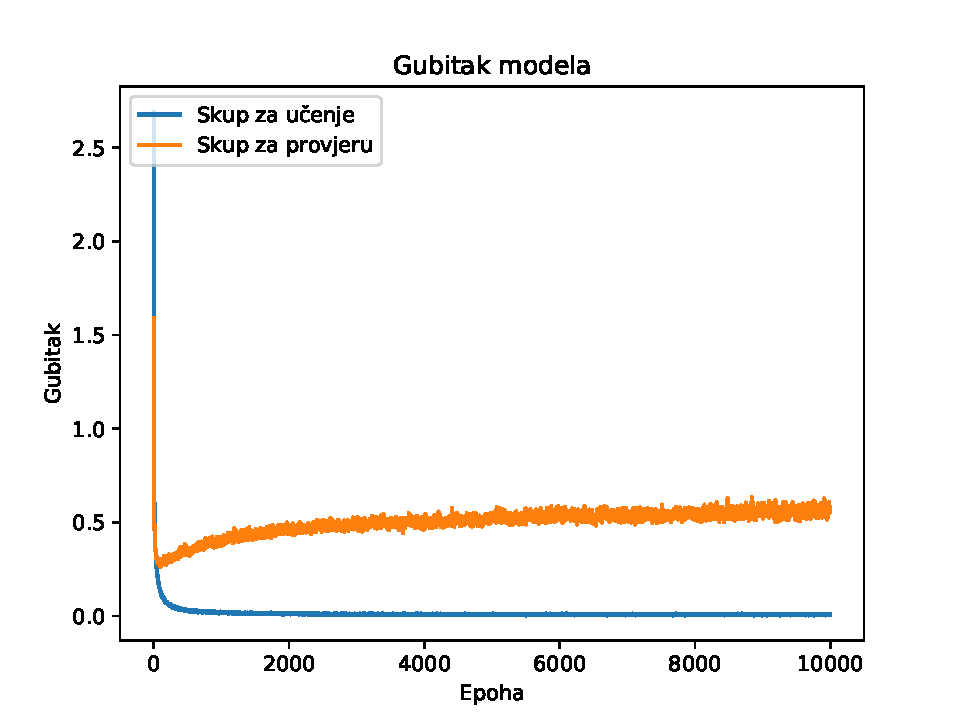
\includegraphics[width=12cm]{images/overfit.pdf}
    \caption{Gubitak prenaučenog modela}
    \label{fig:overfit}
\end{figure}

Kako bi se doskočilo problemu prenaučenosti same mreže, potrebno je uvesti neke regularizacijske tehnike. Najčešće korištena tehnika kod konvolucijskih neuronskih mreža je \emph{dropout} opisana u radu \citep{dropout}. Sam pojam \emph{dropout} se odnosi na ''ispuštanje'' skrivenih ili vanjskih čvorova, u ovom slučaju neurona ili samih filtra konvolucijskog sloja ili sloja sažimanja. ''Ispuštanje'' u kontekstu konvolucijskih neuronskih mreža predstavlja odspajanje pojedinog filtra ili neurona sa svih svojih ulaza i izlaza. Na taj način čvor postaje manje osjetljiv na promjene težina i time se dobiva robusniji model. Sam odabir čvora koji će se ispustiti tokom učenja je slučajan, te sama vjerojatnost ''ispuštanja'' čvora predstavlja hiperparametar modela prilikom faze učenja.

Za arhitekturu konvolucijske neuronske mreže navedenu u prijašnjem potpoglavlju, \emph{dropout} je dodan između zadnjeg sloja sažimanja i prvog potpuno povezanoga sloja i to s vjerojatnošću ispuštanja $0.25$, te između prvog i drugog potpuno povezanoga sloja s vjerojatnošću ispuštanja $0.5$. Tako učena mreža ostvarila je najbolje rezultate. Prikaz vrijednosti funkcije gubitka takve mreže kroz epohe za pojedine skupove vidljiv je na slici \ref{fig:model_loss}, dok se točnost klasifikacije kroz epohe može promatrati na slici \ref{fig:model_acc}.

\begin{figure}[!htbp]
    \centering
    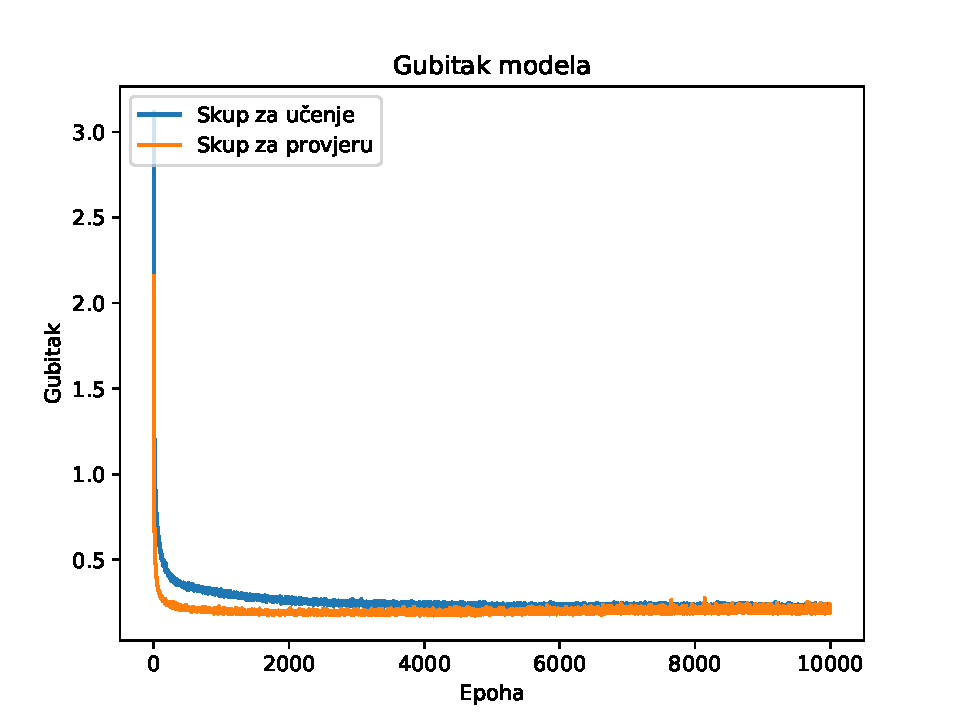
\includegraphics[width=12cm]{images/model_loss.pdf}
    \caption{Gubitak modela}
    \label{fig:model_loss}
\end{figure}

\begin{figure}[!htbp]
    \centering
    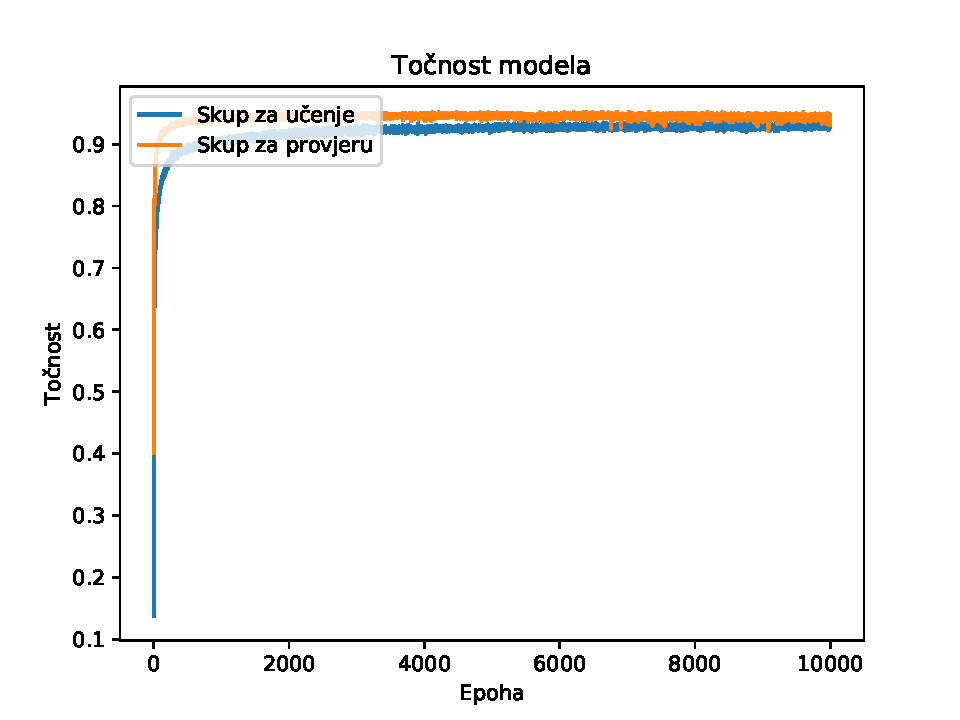
\includegraphics[width=12cm]{images/model_acc.pdf}
    \caption{Točnost klasifikacije modela}
    \label{fig:model_acc}
\end{figure}

\section{Rezultati}

Najbolji rezultati su ostvareni na konvolucijskoj neuronskoj mreži opisanoj u jednom od prijašnjih poglavlja uz već navedene postupke učenja i tehnika regularizacije. Točnost klasifikacije modela na skupu za testiranje iznosila je $94\%$, što znači da je svega $60$ od $1000$ primjera iz skupa za ispitivanje krivo klasificirano.

Primjer krivo klasificiranih primjera iz skupa za ispitivanje vidljiv je na slici \ref{fig:wrong_class}. Može se uočiti kako najviše problema uzrokuju kombinacije malog slova l i velikog slova I, malog slova h i malog slova n, slova u i slova v. No, među danim primjerima se mogu uočiti i krivo napisana slova, poput obrnutog slova N, slova E bez donje crtice i slični. Za velik broj slučajeva s navedene slike ni sam čovjek ne bi mogao točno razlučiti o kojem je slovu riječ bez poznavanja šireg konteksta u kojem se to slovo pojavilo.

\begin{figure}[htb]
    \centering
    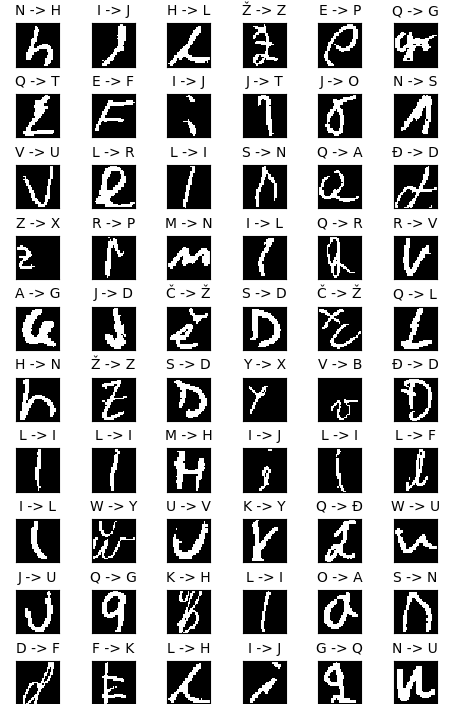
\includegraphics[width=10cm]{images/wrong.png}
    \caption{Krivo klasificirani primjeri iz skupa za ispitivanje. Lijeva strana izraza predstavlja stvarnu oznaku, a desna izlaz klasifikatora.}
    \label{fig:wrong_class}
\end{figure}

Tablicom \ref{confusion_matrix_cro} prikazana je matrica zabune na ispitnom skupu gdje pojedini element iz tablice predstavlja broj koliko je puta slovo iz retka prepoznato kao slovo iz stupca.
 
\begin{table}[]
\setlength{\tabcolsep}{2pt}
\centering
\caption{Matrica zabune za hrvatsku abecedu. Element tablice predstavlja broj koliko je puta slovo iz retka prepoznato kao slovo iz stupca.}
\label{confusion_matrix_cro}
\scalebox{0.75} {
\begin{tabular}{|c|c|c|c|c|c|c|c|c|c|c|c|c|c|c|c|c|c|c|c|c|c|c|c|c|c|c|c|c|c|c|c|c|}
\cline{1-33}
/ & A & B & C & Č & Ć & D & Đ & E & F & G & H & I & J & K & L & M & N & O & P & R & S & Š & T & U & V & Z & Ž & X & Y & W & Q & - \\ \hline \rowcolor{gray1}
A & \textbf{34} & 0 & 0 & 0 & 0 & 0 & 0 & 0 & 0 & 1 & 0 & 0 & 0 & 0 & 0 & 0 & 0 & 0 & 0 & 0 & 0 & 0 & 0 & 0 & 0 & 0 & 0 & 0 & 0 & 0 & 0 & 0 \\ \hline \rowcolor{gray2} 
B & 0 & \textbf{31} & 0 & 0 & 0 & 0 & 0 & 0 & 0 & 0 & 0 & 0 & 0 & 0 & 0 & 0 & 0 & 0 & 0 & 0 & 0 & 0 & 0 & 0 & 0 & 0 & 0 & 0 & 0 & 0 & 0 & 0 \\ \hline \rowcolor{gray1}
C & 0 & 0 & \textbf{29} & 0 & 0 & 0 & 0 & 0 & 0 & 0 & 0 & 0 & 0 & 0 & 0 & 0 & 0 & 0 & 0 & 0 & 0 & 0 & 0 & 0 & 0 & 0 & 0 & 0 & 0 & 0 & 0 & 0 \\ \hline \rowcolor{gray2} 
Č & 0 & 0 & 0 & \textbf{30} & 0 & 0 & 0 & 0 & 0 & 0 & 0 & 0 & 0 & 0 & 0 & 0 & 0 & 0 & 0 & 0 & 0 & 0 & 0 & 0 & 0 & 0 & 2 & 0 & 0 & 0 & 0 & 0 \\ \hline \rowcolor{gray1}
Ć & 0 & 0 & 0 & 0 & \textbf{28} & 0 & 0 & 0 & 0 & 0 & 0 & 0 & 0 & 0 & 0 & 0 & 0 & 0 & 0 & 0 & 0 & 0 & 0 & 0 & 0 & 0 & 0 & 0 & 0 & 0 & 0 & 0 \\ \hline \rowcolor{gray2} 
D & 0 & 0 & 0 & 0 & 0 & \textbf{31} & 0 & 0 & 1 & 0 & 0 & 0 & 0 & 0 & 0 & 0 & 0 & 0 & 0 & 0 & 0 & 0 & 0 & 0 & 0 & 0 & 0 & 0 & 0 & 0 & 0 & 0 \\ \hline \rowcolor{gray1}
Đ & 0 & 0 & 0 & 0 & 0 & 2 & \textbf{27} & 0 & 0 & 0 & 0 & 0 & 0 & 0 & 0 & 0 & 0 & 0 & 0 & 0 & 0 & 0 & 0 & 0 & 0 & 0 & 0 & 0 & 0 & 0 & 0 & 0 \\ \hline \rowcolor{gray2} 
E & 0 & 0 & 0 & 0 & 0 & 0 & 0 & \textbf{31} & 1 & 0 & 0 & 0 & 0 & 0 & 0 & 0 & 0 & 0 & 1 & 0 & 0 & 0 & 0 & 0 & 0 & 0 & 0 & 0 & 0 & 0 & 0 & 0 \\ \hline \rowcolor{gray1}
F & 0 & 0 & 0 & 0 & 0 & 0 & 0 & 0 & \textbf{34} & 0 & 0 & 0 & 0 & 1 & 0 & 0 & 0 & 0 & 0 & 0 & 0 & 0 & 0 & 0 & 0 & 0 & 0 & 0 & 0 & 0 & 0 & 0 \\ \hline \rowcolor{gray2} 
G & 0 & 0 & 0 & 0 & 0 & 0 & 0 & 0 & 0 & \textbf{30} & 0 & 0 & 0 & 0 & 0 & 0 & 0 & 0 & 0 & 0 & 0 & 0 & 0 & 0 & 0 & 0 & 0 & 0 & 0 & 0 & 1 & 0 \\ \hline \rowcolor{gray1}
H & 0 & 0 & 0 & 0 & 0 & 0 & 0 & 0 & 0 & 0 & \textbf{22} & 0 & 0 & 0 & 1 & 0 & 1 & 0 & 0 & 0 & 0 & 0 & 0 & 0 & 0 & 0 & 0 & 0 & 0 & 0 & 0 & 0 \\ \hline \rowcolor{gray2} 
I & 0 & 0 & 0 & 0 & 0 & 0 & 0 & 0 & 0 & 0 & 0 & \textbf{25} & 4 & 0 & 2 & 0 & 0 & 0 & 0 & 0 & 0 & 0 & 0 & 0 & 0 & 0 & 0 & 0 & 0 & 0 & 0 & 0 \\ \hline \rowcolor{gray1}
J & 0 & 0 & 0 & 0 & 0 & 1 & 0 & 0 & 0 & 0 & 0 & 0 & \textbf{21} & 0 & 0 & 0 & 0 & 1 & 0 & 0 & 0 & 0 & 1 & 1 & 0 & 0 & 0 & 0 & 0 & 0 & 0 & 0 \\ \hline \rowcolor{gray2} 
K & 0 & 0 & 0 & 0 & 0 & 0 & 0 & 0 & 0 & 0 & 1 & 0 & 0 & \textbf{32} & 0 & 0 & 0 & 0 & 0 & 0 & 0 & 0 & 0 & 0 & 0 & 0 & 0 & 0 & 1 & 0 & 0 & 0 \\ \hline \rowcolor{gray1}
L & 0 & 0 & 0 & 0 & 0 & 0 & 0 & 0 & 1 & 0 & 1 & 5 & 0 & 0 & \textbf{31} & 0 & 0 & 0 & 0 & 1 & 0 & 0 & 0 & 0 & 0 & 0 & 0 & 0 & 0 & 0 & 0 & 0 \\ \hline \rowcolor{gray2} 
M & 0 & 0 & 0 & 0 & 0 & 0 & 0 & 0 & 0 & 0 & 1 & 0 & 0 & 0 & 0 & \textbf{32} & 1 & 0 & 0 & 0 & 0 & 0 & 0 & 0 & 0 & 0 & 0 & 0 & 0 & 0 & 0 & 0 \\ \hline \rowcolor{gray1}
N & 0 & 0 & 0 & 0 & 0 & 0 & 0 & 0 & 0 & 0 & 1 & 0 & 0 & 0 & 0 & 0 & \textbf{27} & 0 & 0 & 0 & 1 & 0 & 0 & 1 & 0 & 0 & 0 & 0 & 0 & 0 & 0 & 0 \\ \hline \rowcolor{gray2} 
O & 1 & 0 & 0 & 0 & 0 & 0 & 0 & 0 & 0 & 0 & 0 & 0 & 0 & 0 & 0 & 0 & 0 & \textbf{23} & 0 & 0 & 0 & 0 & 0 & 0 & 0 & 0 & 0 & 0 & 0 & 0 & 0 & 0 \\ \hline \rowcolor{gray1}
P & 0 & 0 & 0 & 0 & 0 & 0 & 0 & 0 & 0 & 0 & 0 & 0 & 0 & 0 & 0 & 0 & 0 & 0 & \textbf{26} & 0 & 0 & 0 & 0 & 0 & 0 & 0 & 0 & 0 & 0 & 0 & 0 & 0 \\ \hline \rowcolor{gray2} 
R & 0 & 0 & 0 & 0 & 0 & 0 & 0 & 0 & 0 & 0 & 0 & 0 & 0 & 0 & 0 & 0 & 0 & 0 & 1 & \textbf{35} & 0 & 0 & 0 & 0 & 1 & 0 & 0 & 0 & 0 & 0 & 0 & 0 \\ \hline \rowcolor{gray1}
S & 0 & 0 & 0 & 0 & 0 & 2 & 0 & 0 & 0 & 0 & 0 & 0 & 0 & 0 & 0 & 0 & 2 & 0 & 0 & 0 & \textbf{28} & 0 & 0 & 0 & 0 & 0 & 0 & 0 & 0 & 0 & 0 & 0 \\ \hline \rowcolor{gray2} 
Š & 0 & 0 & 0 & 0 & 0 & 0 & 0 & 0 & 0 & 0 & 0 & 0 & 0 & 0 & 0 & 0 & 0 & 0 & 0 & 0 & 0 & \textbf{45} & 0 & 0 & 0 & 0 & 0 & 0 & 0 & 0 & 0 & 0 \\ \hline \rowcolor{gray1}
T & 0 & 0 & 0 & 0 & 0 & 0 & 0 & 0 & 0 & 0 & 0 & 0 & 0 & 0 & 0 & 0 & 0 & 0 & 0 & 0 & 0 & 0 & \textbf{47} & 0 & 0 & 0 & 0 & 0 & 0 & 0 & 0 & 0 \\ \hline \rowcolor{gray2} 
U & 0 & 0 & 0 & 0 & 0 & 0 & 0 & 0 & 0 & 0 & 0 & 0 & 0 & 0 & 0 & 0 & 0 & 0 & 0 & 0 & 0 & 0 & 0 & \textbf{26} & 1 & 0 & 0 & 0 & 0 & 0 & 0 & 0 \\ \hline \rowcolor{gray1}
V & 0 & 1 & 0 & 0 & 0 & 0 & 0 & 0 & 0 & 0 & 0 & 0 & 0 & 0 & 0 & 0 & 0 & 0 & 0 & 0 & 0 & 0 & 0 & 1 & \textbf{30} & 0 & 0 & 0 & 0 & 0 & 0 & 0 \\ \hline \rowcolor{gray2} 
Z & 0 & 0 & 0 & 0 & 0 & 0 & 0 & 0 & 0 & 0 & 0 & 0 & 0 & 0 & 0 & 0 & 0 & 0 & 0 & 0 & 0 & 0 & 0 & 0 & 0 & \textbf{26} & 0 & 1 & 0 & 0 & 0 & 0 \\ \hline \rowcolor{gray1}
Ž & 0 & 0 & 0 & 0 & 0 & 0 & 0 & 0 & 0 & 0 & 0 & 0 & 0 & 0 & 0 & 0 & 0 & 0 & 0 & 0 & 0 & 0 & 0 & 0 & 0 & 2 & \textbf{26} & 0 & 0 & 0 & 0 & 0 \\ \hline \rowcolor{gray2} 
X & 0 & 0 & 0 & 0 & 0 & 0 & 0 & 0 & 0 & 0 & 0 & 0 & 0 & 0 & 0 & 0 & 0 & 0 & 0 & 0 & 0 & 0 & 0 & 0 & 0 & 0 & 0 & \textbf{29} & 0 & 0 & 0 & 0 \\ \hline \rowcolor{gray1}
Y & 0 & 0 & 0 & 0 & 0 & 0 & 0 & 0 & 0 & 0 & 0 & 0 & 0 & 0 & 0 & 0 & 0 & 0 & 0 & 0 & 0 & 0 & 0 & 0 & 0 & 0 & 0 & 1 & \textbf{23} & 0 & 0 & 0 \\ \hline \rowcolor{gray2} 
W & 0 & 0 & 0 & 0 & 0 & 0 & 0 & 0 & 0 & 0 & 0 & 0 & 0 & 0 & 0 & 0 & 0 & 0 & 0 & 0 & 0 & 0 & 0 & 1 & 0 & 0 & 0 & 0 & 1 & \textbf{23} & 0 & 0 \\ \hline \rowcolor{gray1}
Q & 1 & 0 & 0 & 0 & 0 & 0 & 1 & 0 & 0 & 2 & 0 & 0 & 0 & 0 & 1 & 0 & 0 & 0 & 0 & 1 & 0 & 0 & 1 & 0 & 0 & 0 & 0 & 0 & 0 & 0 & \textbf{23} & 0 \\ \hline \rowcolor{gray2} 
- & 0 & 0 & 0 & 0 & 0 & 0 & 0 & 0 & 0 & 0 & 0 & 0 & 0 & 0 & 0 & 0 & 0 & 0 & 0 & 0 & 0 & 0 & 0 & 0 & 0 & 0 & 0 & 0 & 0 & 0 & 0 & \textbf{35} \\ \hline
\end{tabular}
}
\end{table}

\chapter{Zaključak}
Tehnika očitavanja rukom pisanih slova se razvija još od polovice prošlog stoljeća i od tada je u mnogočemu evoluirala. U ovom radu, kao klasifikator pojedinog slova, korištena je konvolucijska neuronska mreža.

U radu je predstavljen cjeloviti postupak prikupljanja skupa podataka i obrade slike kako bi se ulazna slika pripremila za svrhu učenja konvolucijske neuronske mreže. Također, opisana je arhitektura korištene neuronske mreže i postupak učenja iste.

Dobiveni rezultati su vrlo zadovoljavajući za dani skup podataka. Usporedbe radi, u radu \citep{zavrsni} prikazana je obična neuronska mreža učena na nešto manjem skupu podataka uz ručno izlučivanje značajki, te je dobivena točnost klasifikatora za hrvatsku abecedu iznosila $78.44\%$.

Konvolucijske neuronske mreže su se pokazale kao iznimno dobar klasifikator u području klasificiranja slike. U budućnosti bi se mogao proširiti sam skup podataka te bi se kao klasifikator mogle isprobati nešto kompliciranije konvolucijske neuronske mreže učene naprednijim algoritmima učenja, poput one navedene u radu \citep{lenet5hecr}.


\bibliography{literatura}
\bibliographystyle{fer}

\chapter{Sažetak}
U ovom radu opisana je implementacija i način rada sustav za očitavanje rukom pisanih slova koji je projektiran tako da na svoj ulaz primi sliku slova dimenzija $30 \times 30$, a na svom izlazu vrati prepoznato slovo. Sam sustav je zasnovan na konvolucijskoj neuronskoj mreži učenu metodom \emph{ADADELTA}. Skup za učenje konvolucijske neuronske mreže se sastojao od \num{12,000} velikih i malih tiskanih slova hrvatske i engleske abecede te znaka ''-''. Točnost klasifikatora provjerena je na skupu za ispitivanje koji se sastojao od \num{1000} znakova te je iznosila $94 \%$.

\end{document}
